\section{Panoramic image reconstruction}

Panoramic images offer a wide-angle perspective of scenes through the seamless merging of multiple images taken from different viewpoints. This process involves several key steps, including the extraction of key point features, their matching, and the estimation of homographies.

Key point feature extraction techniques like Scale-Invariant Feature Transform (SIFT) or Features from Accelerated Segment Test (FAST) play crucial roles in panoramic image stitching. These techniques identify distinctive points or regions in images that remain invariant to changes in scale, rotation, and illumination. Robust features are extracted from each image to enable subsequent matching of corresponding points across overlapping images.

Following key point extraction, the matching process aims to establish correspondences between these points across different images (Fig. \ref{fig:homog_example}).

\begin{figure}[H]
    \centering
    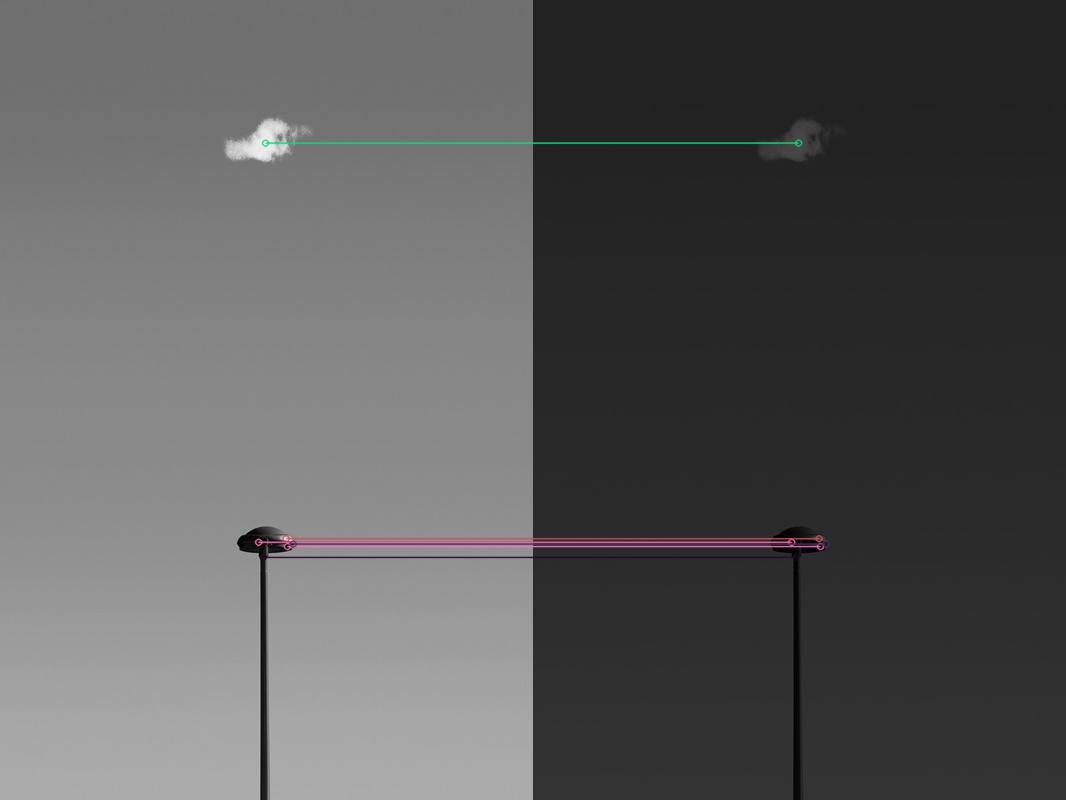
\includegraphics[width=0.4\textwidth]{../sift_algorithm/img/final.png}
    \caption{Example of key point matching}
    \label{fig:homog_example}
\end{figure}

Homography estimation is then performed to calculate the transformation necessary to align matched key points between images. Estimating the homography matrix enables effective warping and blending of images to produce a seamless panoramic composition (Fig. \ref{fig:pano}). 

\begin{figure}[H]
    \centering
    \subfloat[Original images before the mosaic \cite{gledhill_panoramic_2003}]{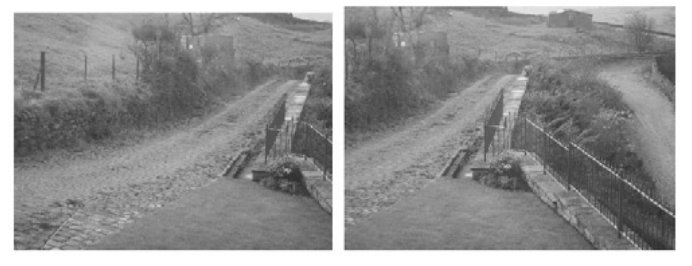
\includegraphics[width=0.4\textwidth]{img/pano_both.png}} \qquad
    \subfloat[Two images stitched together \cite{gledhill_panoramic_2003}]{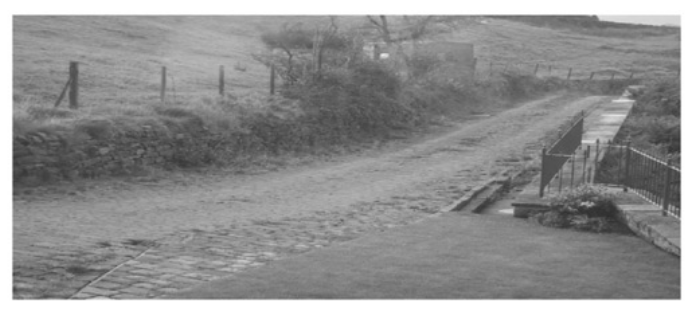
\includegraphics[width=0.35\textwidth]{img/pano_join.png}}
    \caption{Example of panoramic image reconstruction}
    \label{fig:pano}
\end{figure}
